\documentclass{article}
\usepackage{tikz}
\usepackage{amsmath, amssymb}
\usetikzlibrary{calc}
\usepgflibrary{fpu}
\begin{document}

\begin{enumerate}

	\item Draw the following vectors in standard position in R$^{2}$

	\begin{enumerate}

	\item $\text{a } = \begin{bmatrix} 3 \\ 0 \\ \end{bmatrix} $

	\item $\text{b } = \begin{bmatrix} 2 \\ 3 \\ \end{bmatrix} $

	\item $\text{c } = \begin{bmatrix} -2 \\ 3 \\ \end{bmatrix}$

	\item $\text{d } = \begin{bmatrix} 3 \\ -2 \\ \end{bmatrix}$

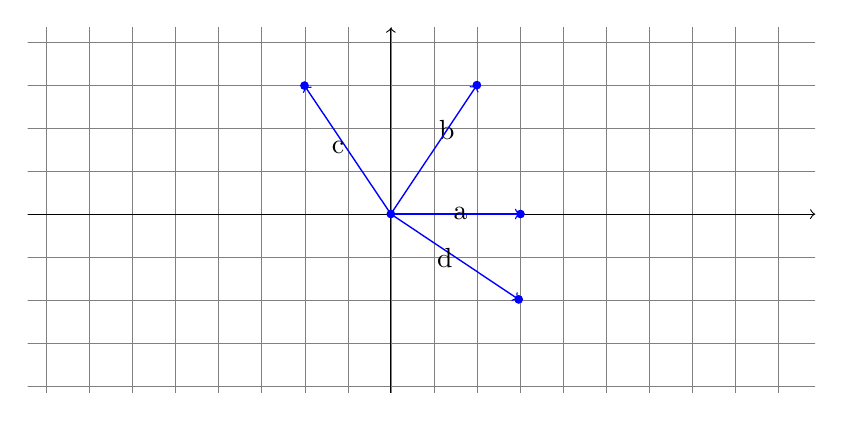
\begin{tikzpicture}[%
scale=0.546427,
]
\clip (-8.44094,-4.15788) rectangle (9.85978,4.33184);
\draw [help lines] (0,0) grid (10,5);
\draw [help lines] (-9,0) grid (0,5);
\draw [help lines] (0,-5) grid (10,0);
\draw [help lines] (-9,-5) grid (0,0);
\draw [color=black,->] (-8.44094,0) -- (9.85978,0);
\draw [color=black,->] (0,-4.15788) -- (0,4.33184);
%% point;
\filldraw [color={rgb:red,0;green,0;blue,255}] (1.99927,2.99627) circle (2.5pt );
%% vector;
\draw[color={rgb:red,0;green,0;blue,255}, line width=0.5pt, solid, ->] (0,0.000547801) -- (3.01218,0.000547801);
%% point;
\filldraw [color={rgb:red,0;green,0;blue,255}] (2.97045,-1.98382) circle (2.5pt );
%% point;
\filldraw [color={rgb:red,0;green,0;blue,255}] (0,0.000547801) circle (2.5pt );
%% vector;
\draw[color={rgb:red,0;green,0;blue,255}, line width=0.5pt, solid, ->] (0,0.000547801) -- (-2.00686,2.98488);
%% point;
\filldraw [color={rgb:red,0;green,0;blue,255}] (-2.00686,2.98488) circle (2.5pt );
%% label;
\node at (1.61303,0.000547801) {a};
%% point;
\filldraw [color={rgb:red,0;green,0;blue,255}] (3.01218,0.000547801) circle (2.5pt );
%% label;
\node at (1.30014,1.94869) {b};
%% vector;
\draw[color={rgb:red,0;green,0;blue,255}, line width=0.5pt, solid, ->] (0,0.000547801) -- (2.97045,-1.98382);
%% label;
\node at (1.25574,-1.02064) {d};
%% vector;
\draw[color={rgb:red,0;green,0;blue,255}, line width=0.5pt, solid, ->] (0,0.000547801) -- (1.99927,2.99627);
%% label;
\node at (-1.22843,1.55652) {c};
\end{tikzpicture}

	\end{enumerate}

	\item Draw the vectors in Exercise 1 with their tails at the
		point (1, -3).

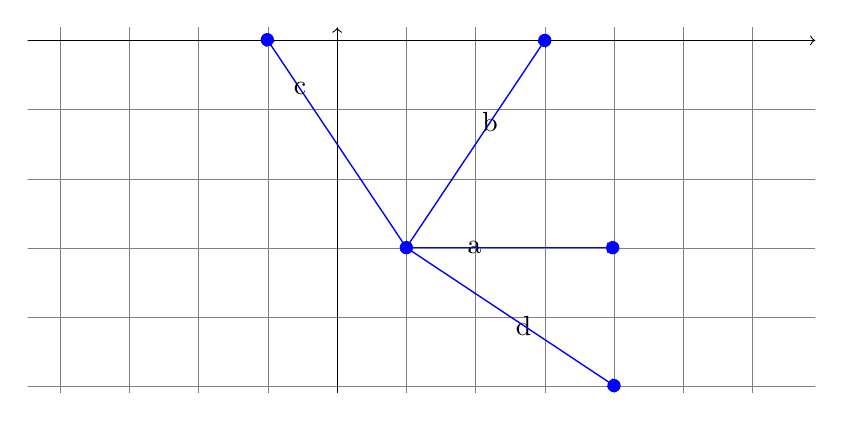
\begin{tikzpicture}[%
scale=0.879603,
]
\clip (-4.46832,-5.09049) rectangle (6.90044,0.183483);
\draw [help lines] (0,0) grid (7,1);
\draw [help lines] (-5,0) grid (0,1);
\draw [help lines] (0,-6) grid (7,0);
\draw [help lines] (-5,-6) grid (0,0);
\draw [color=black,->] (-4.46832,0) -- (6.90044,0);
\draw [color=black,->] (0,-5.09049) -- (0,0.183483);
%% label;
\node at (1.97963,-2.99268) {a};
%% point;
\filldraw [color={rgb:red,0;green,0;blue,255}] (0.999244,-2.99268) circle (2.5pt );
%% vector;
\draw[color={rgb:red,0;green,0;blue,255}, line width=0.5pt, solid, ->] (0.999244,-2.99268) -- (2.99773,-8.88178e-4);
%% vector;
\draw[color={rgb:red,0;green,0;blue,255}, line width=0.5pt, solid, ->] (0.999244,-2.99268) -- (3.97812,-2.99268);
%% point;
\filldraw [color={rgb:red,0;green,0;blue,255}] (3.97812,-2.99268) circle (2.5pt );
%% label;
\node at (2.6903,-4.11616) {d};
%% vector;
\draw[color={rgb:red,0;green,0;blue,255}, line width=0.5pt, solid, ->] (0.999244,-2.99268) -- (-1.00867,0.00942683);
%% point;
\filldraw [color={rgb:red,0;green,0;blue,255}] (2.99773,-8.88178e-4) circle (2.5pt );
%% label;
\node at (2.20786,-1.18281) {b};
%% point;
\filldraw [color={rgb:red,0;green,0;blue,255}] (-1.00867,0.00942683) circle (2.5pt );
%% vector;
\draw[color={rgb:red,0;green,0;blue,255}, line width=0.5pt, solid, ->] (0.999244,-2.99268) -- (3.99698,-4.98427);
%% point;
\filldraw [color={rgb:red,0;green,0;blue,255}] (3.99698,-4.98427) circle (2.5pt );
%% label;
\node at (-0.537741,-0.694678) {c};
\end{tikzpicture}

	\item Draw the following vectors in standard position in R$^{3}$.

	\begin{enumerate}
		\item $\text{a } = \begin{bmatrix} 0, & 2, & 1 \end{bmatrix}$

		\item $\text{b } = \begin{bmatrix} 3, & 2, & 1 \end{bmatrix}$

		\item $\text{c } = \begin{bmatrix} 1, & -2, 1 \end{bmatrix}$

		\item $\text{d } = \begin{bmatrix} -1, & -1, & -2 \end{bmatrix}$
	\end{enumerate}

	\item If the vectors in Exercise 3 are translated so that their
		heads are at the point $(1, 2, 3)$, find the points that
		correspond to their tails.

	\begin{enumerate}

		\item $\text{a } = (1,0,2)$

		\item $\text{b } = (-2,0,2)$

		\item $\text{c } = (0,4,2)$

		\item $\text{d } = (2,3,5)$

	\end{enumerate}

	\item For each of the following pairs of points, draw the vector AB.
		Then compute and redraw AB as a vector in standard position.

	\begin{enumerate}
		\item $A = (1,-1), B = (4,2)$

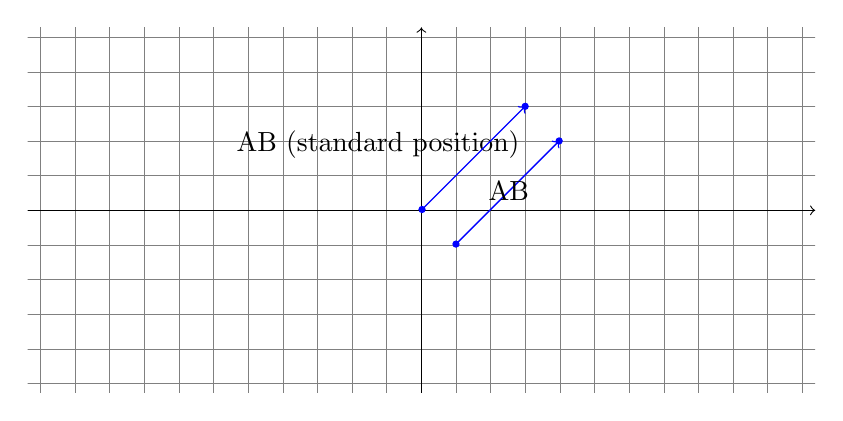
\begin{tikzpicture}[%
scale=0.439802,
]
\clip (-11.3688,-5.27397) rectangle (11.3688,5.27397);
\draw [help lines] (0,0) grid (12,6);
\draw [help lines] (-12,0) grid (0,6);
\draw [help lines] (0,-6) grid (12,0);
\draw [help lines] (-12,-6) grid (0,0);
\draw [color=black,->] (-11.3688,0) -- (11.3688,0);
\draw [color=black,->] (0,-5.27397) -- (0,5.27397);
%% point;
\filldraw [color={rgb:red,0;green,0;blue,255}] (3.97812,2.00354) circle (2.5pt );
%% label;
\node at (-1.25377,1.89985) {AB (standard position)};
%% vector;
\draw[color={rgb:red,0;green,0;blue,255}, line width=0.5pt, solid, ->] (0.0188537,0.0239074) -- (2.99773,3.00279);
%% vector;
\draw[color={rgb:red,0;green,0;blue,255}, line width=0.5pt, solid, ->] (0.999244,-0.975337) -- (3.97812,2.00354);
%% point;
\filldraw [color={rgb:red,0;green,0;blue,255}] (0.0188537,0.0239074) circle (2.5pt );
%% label;
\node at (2.52639,0.55181) {AB};
%% point;
\filldraw [color={rgb:red,0;green,0;blue,255}] (2.99773,3.00279) circle (2.5pt );
%% point;
\filldraw [color={rgb:red,0;green,0;blue,255}] (0.999244,-0.975337) circle (2.5pt );
\end{tikzpicture}

	\item $A = (0,-2), B = (2,-1)$

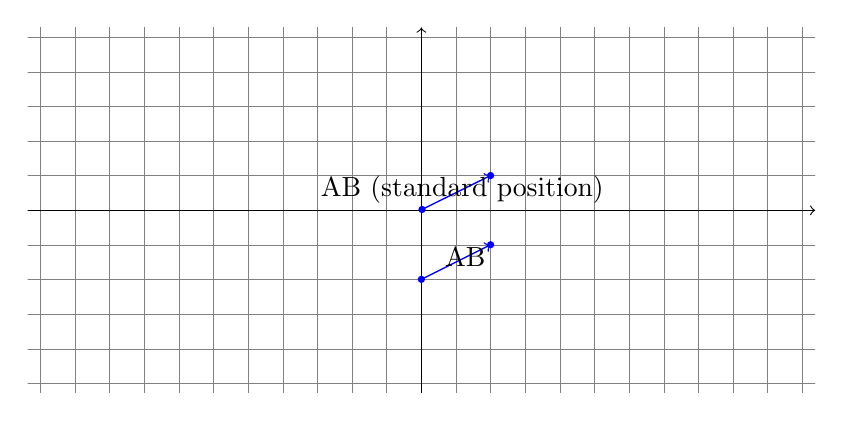
\begin{tikzpicture}[%
scale=0.439802,
]
\clip (-11.3688,-5.27397) rectangle (11.3688,5.27397);
\draw [help lines] (0,0) grid (12,6);
\draw [help lines] (-12,0) grid (0,6);
\draw [help lines] (0,-6) grid (12,0);
\draw [help lines] (-12,-6) grid (0,0);
\draw [color=black,->] (-11.3688,0) -- (11.3688,0);
\draw [color=black,->] (0,-5.27397) -- (0,5.27397);
%% point;
\filldraw [color={rgb:red,0;green,0;blue,255}] (1.99849,1.0043) circle (2.5pt );
%% point;
\filldraw [color={rgb:red,0;green,0;blue,255}] (0,-1.99343) circle (2.5pt );
%% vector;
\draw[color={rgb:red,0;green,0;blue,255}, line width=0.5pt, solid, ->] (0,-1.99343) -- (1.99849,-0.994191);
%% vector;
\draw[color={rgb:red,0;green,0;blue,255}, line width=0.5pt, solid, ->] (0.0188537,0.0239074) -- (1.99849,1.0043);
%% point;
\filldraw [color={rgb:red,0;green,0;blue,255}] (1.99849,-0.994191) circle (2.5pt );
%% label;
\node at (1.26697,-1.35995) {AB};
%% point;
\filldraw [color={rgb:red,0;green,0;blue,255}] (0.0188537,0.0239074) circle (2.5pt );
%% label;
\node at (1.18235,0.600116) {AB (standard position)};
\end{tikzpicture}

	\item $A = (2, \frac{3}{2}), B = (\frac{1}{2},3)$

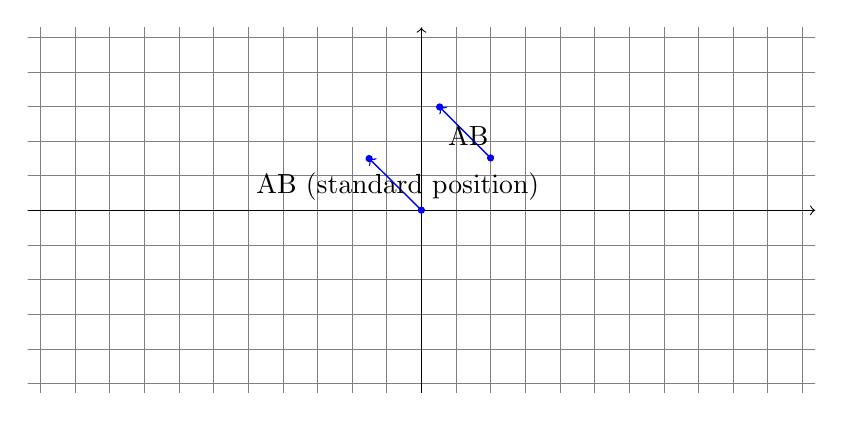
\begin{tikzpicture}[%
scale=0.439802,
]
\clip (-11.3688,-5.27397) rectangle (11.3688,5.27397);
\draw [help lines] (0,0) grid (12,6);
\draw [help lines] (-12,0) grid (0,6);
\draw [help lines] (0,-6) grid (12,0);
\draw [help lines] (-12,-6) grid (0,0);
\draw [color=black,->] (-11.3688,0) -- (11.3688,0);
\draw [color=black,->] (0,-5.27397) -- (0,5.27397);
%% vector;
\draw[color={rgb:red,0;green,0;blue,255}, line width=0.5pt, solid, ->] (0,0.00505372) -- (-1.50829,1.49449);
%% point;
\filldraw [color={rgb:red,0;green,0;blue,255}] (0.527903,2.98393) circle (2.5pt );
%% point;
\filldraw [color={rgb:red,0;green,0;blue,255}] (-1.50829,1.49449) circle (2.5pt );
%% point;
\filldraw [color={rgb:red,0;green,0;blue,255}] (1.99849,1.51335) circle (2.5pt );
%% point;
\filldraw [color={rgb:red,0;green,0;blue,255}] (0,0.00505372) circle (2.5pt );
%% label;
\node at (-0.682974,0.67949) {AB (standard position)};
%% vector;
\draw[color={rgb:red,0;green,0;blue,255}, line width=0.5pt, solid, ->] (1.99849,1.51335) -- (0.527903,2.98393);
%% label;
\node at (1.35746,2.15437) {AB};
\end{tikzpicture}

	\item $A = (\frac{1}{3},\frac{1}{3}),B = (\frac{1}{6},\frac{1}{2})$

\begin{tikzpicture}[%
scale=3.51841,
]
\clip (-1.4211,-0.419203) rectangle (1.4211,0.899291);
\draw [help lines] (0,0) grid (2,1);
\draw [help lines] (-2,0) grid (0,1);
\draw [help lines] (0,-1) grid (2,0);
\draw [help lines] (-2,-1) grid (0,0);
\draw [color=black,->] (-1.4211,0) -- (1.4211,0);
\draw [color=black,->] (0,-0.419203) -- (0,0.899291);
%% vector;
\draw[color={rgb:red,0;green,0;blue,255}, line width=0.5pt, solid, ->] (0,0.00029141) -- (-0.176753,0.181758);
%% point;
\filldraw [color={rgb:red,0;green,0;blue,255}] (0.329939,0.332587) circle (0.5pt );
%% label;
\node at (-0.0825327,0.085025) {AB (standard position)};
%% point;
\filldraw [color={rgb:red,0;green,0;blue,255}] (-0.176753,0.181758) circle (0.5pt );
%% label;
\node at (0.259746,0.400884) {AB};
%% vector;
\draw[color={rgb:red,0;green,0;blue,255}, line width=0.5pt, solid, ->] (0.329939,0.332587) -- (0.155543,0.50227);
%% point;
\filldraw [color={rgb:red,0;green,0;blue,255}] (0.155543,0.50227) circle (0.5pt );
%% point;
\filldraw [color={rgb:red,0;green,0;blue,255}] (0,0.00029141) circle (0.5pt );
\end{tikzpicture}

	\end{enumerate}

	\item A hiker walks 4km north and then 5km northeast. Draw displacement
	vectors representing the hiker's trip and draw a vector that
	represents the hiker's net displacement from the starting point.

	For 5km north-east, the north and east components are $5\cos(45)= 3.53...$

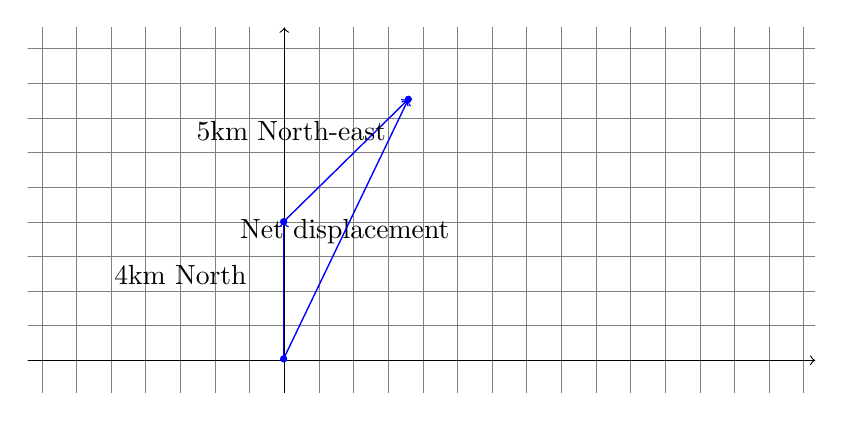
\begin{tikzpicture}[%
scale=0.439802,
]
\clip (-7.40949,-0.942683) rectangle (15.328,9.60526);
\draw [help lines] (0,0) grid (16,10);
\draw [help lines] (-8,0) grid (0,10);
\draw [help lines] (0,-1) grid (16,0);
\draw [help lines] (-8,-1) grid (0,0);
\draw [color=black,->] (-7.40949,0) -- (15.328,0);
\draw [color=black,->] (0,-0.942683) -- (0,9.60526);
%% point;
\filldraw [color={rgb:red,0;green,0;blue,255}] (-0.0188537,0.0427611) circle (2.5pt );
%% vector;
\draw[color={rgb:red,0;green,0;blue,255}, line width=0.5pt, solid, ->] (-0.0188537,4.00203) -- (3.5822,7.53777);
%% label;
\node at (1.74701,3.71812) {Net displacement};
%% label;
\node at (-2.99773,2.47169) {4km North};
%% label;
\node at (0.203557,6.62744) {5km North-east};
%% point;
\filldraw [color={rgb:red,0;green,0;blue,255}] (-0.0188537,4.00203) circle (2.5pt );
%% vector;
\draw[color={rgb:red,0;green,0;blue,255}, line width=0.5pt, solid, ->] (-0.0188537,0.0427611) -- (3.5822,7.53777);
%% vector;
\draw[color={rgb:red,0;green,0;blue,255}, line width=0.5pt, solid, ->] (-0.0188537,0.0427611) -- (-0.0188537,4.00203);
%% point;
\filldraw [color={rgb:red,0;green,0;blue,255}] (3.5822,7.53777) circle (2.5pt );
\end{tikzpicture}

	\emph{Exercises 7-10 refer to the vectors in Exercise 1. Compute
		the indicated vectors and also show how the vectors can
		be obtained geometrically.}

	\item $\text{d } - \text{ c}$

		$$\begin{bmatrix} 3 \\ -2 \\ \end{bmatrix} - \begin{bmatrix} -2 \\ 3 \\ \end{bmatrix}$$

		$$\begin{bmatrix} 3 - (-2) \\ -2 - 3 \\ \end{bmatrix} = \begin{bmatrix} 5 \\ -5 \\ \end{bmatrix}$$

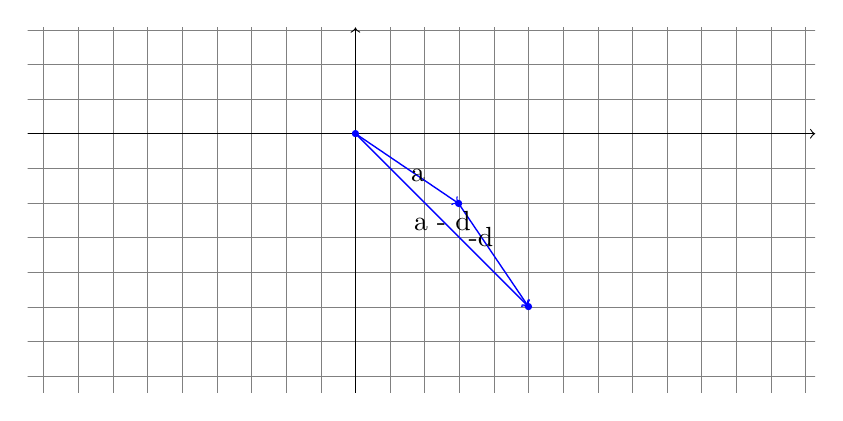
\begin{tikzpicture}[%
scale=0.439802,
]
\clip (-9.46454,-7.48491) rectangle (13.273,3.06304);
\draw [help lines] (0,0) grid (14,4);
\draw [help lines] (-10,0) grid (0,4);
\draw [help lines] (0,-8) grid (14,0);
\draw [help lines] (-10,-8) grid (0,0);
\draw [color=black,->] (-9.46454,0) -- (13.273,0);
\draw [color=black,->] (0,-7.48491) -- (0,3.06304);
%% point;
\filldraw [color={rgb:red,0;green,0;blue,255}] (4.99622,-4.99117) circle (2.5pt );
%% vector;
\draw[color={rgb:red,0;green,0;blue,255}, line width=0.5pt, solid, ->] (2.97888,-2.01229) -- (4.99622,-4.99117);
%% label;
\node at (3.62403,-2.96494) {-d};
%% point;
\filldraw [color={rgb:red,0;green,0;blue,255}] (0,0.00505372) circle (2.5pt );
%% label;
\node at (2.50754,-2.50248) {a - d};
%% vector;
\draw[color={rgb:red,0;green,0;blue,255}, line width=0.5pt, solid, ->] (0,0.00505372) -- (4.99622,-4.99117);
%% point;
\filldraw [color={rgb:red,0;green,0;blue,255}] (2.97888,-2.01229) circle (2.5pt );
%% vector;
\draw[color={rgb:red,0;green,0;blue,255}, line width=0.5pt, solid, ->] (0,0.00505372) -- (2.97888,-2.01229);
%% label;
\node at (1.80109,-1.21467) {a};
\end{tikzpicture}

	\item $\text{a } - \text{ d}$

		$$\begin{bmatrix} 3 \\ 0 \\ \end{bmatrix} - \begin{bmatrix} 3 \\ -2 \\ \end{bmatrix}$$

		$$\begin{bmatrix} 3 - 3 \\ 0 - (-2) \\ \end{bmatrix} = \begin{bmatrix} 0 \\ 2 \\ \end{bmatrix}$$

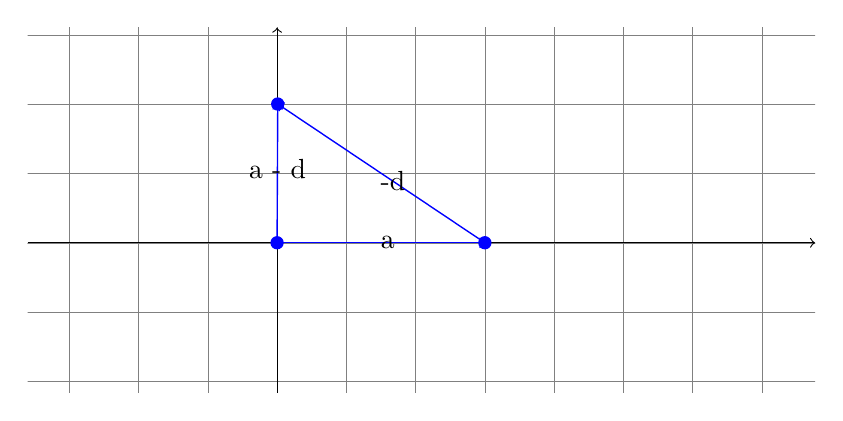
\begin{tikzpicture}[%
scale=0.879603,
]
\clip (-3.60105,-2.16817) rectangle (7.76771,3.1058);
\draw [help lines] (0,0) grid (8,4);
\draw [help lines] (-4,0) grid (0,4);
\draw [help lines] (0,-3) grid (8,0);
\draw [help lines] (-4,-3) grid (0,0);
\draw [color=black,->] (-3.60105,0) -- (7.76771,0);
\draw [color=black,->] (0,-2.16817) -- (0,3.1058);
%% point;
\filldraw [color={rgb:red,0;green,0;blue,255}] (3.00009,0.000340305) circle (2.5pt );
%% vector;
\draw[color={rgb:red,0;green,0;blue,255}, line width=0.5pt, solid, ->] (0,0.000340305) -- (3.00009,0.000340305);
%% vector;
\draw[color={rgb:red,0;green,0;blue,255}, line width=0.5pt, solid, ->] (3.00009,0.000340305) -- (0.00942683,2.00354);
%% label;
\node at (1.67203,0.889902) {-d};
%% point;
\filldraw [color={rgb:red,0;green,0;blue,255}] (0,0.000340305) circle (2.5pt );
%% vector;
\draw[color={rgb:red,0;green,0;blue,255}, line width=0.5pt, solid, ->] (0,0.000340305) -- (0.00942683,2.00354);
%% label;
\node at (0.00499156,1.06105) {a - d};
%% label;
\node at (1.59313,0.000340305) {a};
%% point;
\filldraw [color={rgb:red,0;green,0;blue,255}] (0.00942683,2.00354) circle (2.5pt );
\end{tikzpicture}

	\item $\text{a } + \text{ b}$

		$$\begin{bmatrix} 3 \\ 0 \\ \end{bmatrix} + \begin{bmatrix} 2 \\ 3 \\ \end{bmatrix}$$

		$$\begin{bmatrix}3 + 2 \\ 0 + 3 \\ \end{bmatrix} = \begin{bmatrix} 5 \\ 3 \\ \end{bmatrix}$$

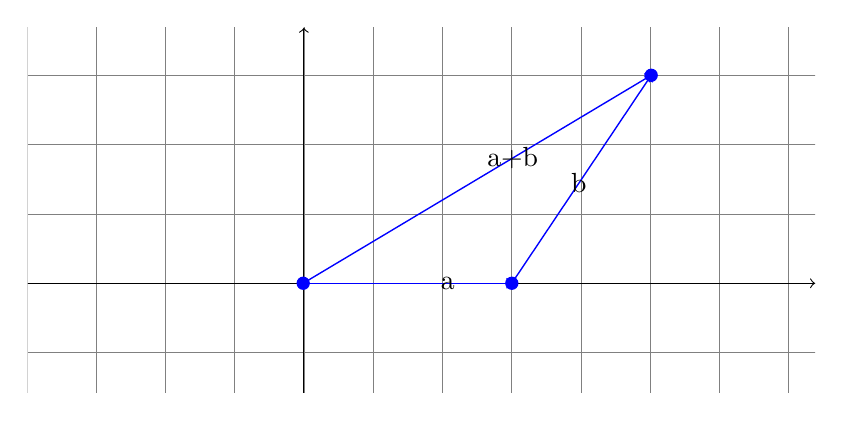
\begin{tikzpicture}[%
scale=0.879603,
]
\clip (-3.98755,-1.58371) rectangle (7.38121,3.69026);
\draw [help lines] (0,0) grid (8,4);
\draw [help lines] (-4,0) grid (0,4);
\draw [help lines] (0,-2) grid (8,0);
\draw [help lines] (-4,-2) grid (0,0);
\draw [color=black,->] (-3.98755,0) -- (7.38121,0);
\draw [color=black,->] (0,-1.58371) -- (0,3.69026);
%% point;
\filldraw [color={rgb:red,0;green,0;blue,255}] (-0.00942683,0.000340305) circle (2.5pt );
%% vector;
\draw[color={rgb:red,0;green,0;blue,255}, line width=0.5pt, solid, ->] (3.00245,0.000340305) -- (5.01508,3.00279);
%% point;
\filldraw [color={rgb:red,0;green,0;blue,255}] (5.01508,3.00279) circle (2.5pt );
%% vector;
\draw[color={rgb:red,0;green,0;blue,255}, line width=0.5pt, solid, ->] (-0.00942683,0.000340305) -- (3.00245,0.000340305);
%% vector;
\draw[color={rgb:red,0;green,0;blue,255}, line width=0.5pt, solid, ->] (-0.00942683,0.000340305) -- (5.01508,3.00279);
%% label;
\node at (2.0739,0.000340305) {a};
%% point;
\filldraw [color={rgb:red,0;green,0;blue,255}] (3.00245,0.000340305) circle (2.5pt );
%% label;
\node at (3.96983,1.44349) {b};
%% label;
\node at (3.01383,1.80692) {a+b};
\end{tikzpicture}

	\item $\text{b } + \text{ c}$

		$$\begin{bmatrix} 2 \\ 3 \\ \end{bmatrix} + \begin{bmatrix} -2 \\ 3 \\ \end{bmatrix}$$

		$$\begin{bmatrix} 2 + (-2) \\ 3 + 3 \\ \end{bmatrix} = \begin{bmatrix} 0 \\ 6 \\ \end{bmatrix}$$

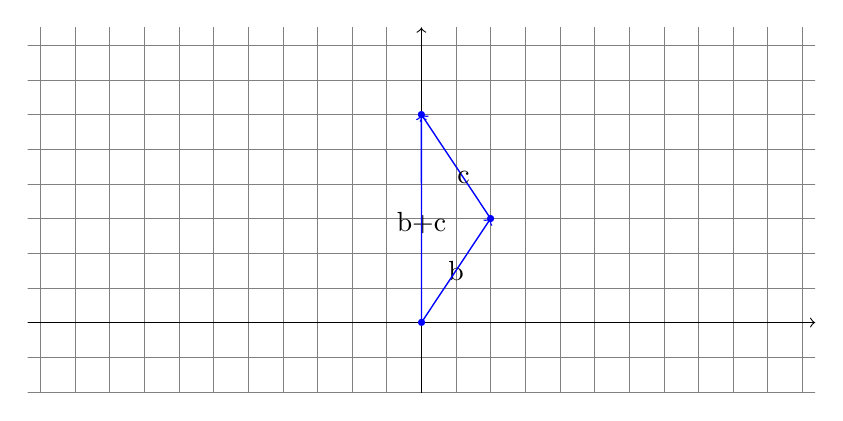
\begin{tikzpicture}[%
scale=0.439802,
]
\clip (-11.3688,-2.03367) rectangle (11.3688,8.51428);
\draw [help lines] (0,0) grid (12,9);
\draw [help lines] (-12,0) grid (0,9);
\draw [help lines] (0,-3) grid (12,0);
\draw [help lines] (-12,-3) grid (0,0);
\draw [color=black,->] (-11.3688,0) -- (11.3688,0);
\draw [color=black,->] (0,-2.03367) -- (0,8.51428);
%% point;
\filldraw [color={rgb:red,0;green,0;blue,255}] (4.44089e-4,6.00557) circle (2.5pt );
%% point;
\filldraw [color={rgb:red,0;green,0;blue,255}] (0.00471342,0.00505372) circle (2.5pt );
%% label;
\node at (0.00245827,2.87601) {b+c};
%% label;
\node at (0.999658,1.501) {b};
%% vector;
\draw[color={rgb:red,0;green,0;blue,255}, line width=0.5pt, solid, ->] (1.99849,3.00279) -- (4.44089e-4,6.00557);
%% vector;
\draw[color={rgb:red,0;green,0;blue,255}, line width=0.5pt, solid, ->] (0.00471342,0.00505372) -- (1.99849,3.00279);
%% label;
\node at (1.21825,4.17511) {c};
%% point;
\filldraw [color={rgb:red,0;green,0;blue,255}] (1.99849,3.00279) circle (2.5pt );
%% vector;
\draw[color={rgb:red,0;green,0;blue,255}, line width=0.5pt, solid, ->] (0.00471342,0.00505372) -- (4.44089e-4,6.00557);
\end{tikzpicture}

	\emph{Exercises 11 and 12 refer to the vectors in Exercise 3. Compute the indicated vectors.}

	\item $2\boldsymbol{a} + 3\boldsymbol{c}$

		$$2[0, 2, 0] + 3[1, -2, 1]$$
		$$[0, 4, 0] + [3, -6, 3]$$
		$$[0 + 3, 4 + (-6), 0 + 3] = [3, -2, 3]$$

	\item $2\boldsymbol{c} - 3\boldsymbol{b} - d$

		$$2[1, -2, 1] - 3[3, 2, 1] - [-1, -1, -2]$$

		$$[2, -4, 2] - [9, 6, 3] - [-1, -1, -2]$$

		$$[2-9-(-1),(-4)-6-(-1),2-3-(-2)] = [-6,-9,1]$$

	\item Find the components of vectors $\boldsymbol{u}, \boldsymbol{v}, \boldsymbol{u} +
		\boldsymbol{v}, \text{ and } \boldsymbol{u} - \boldsymbol{v}$, where u and v
		are as shown in Figure 1.23.

		$\boldsymbol{u} = [\sin 60, \cos 60] = [\sqrt{3}/2, 1/2]$

		$\boldsymbol{v} = [-\sin 30, - \cos 30] = [- 1/2, - \sqrt{3}/2]$

		$\boldsymbol{u} + \boldsymbol{v} = [\sqrt{3}/2 - 1/2, 1/2 - \sqrt{3}/2] = [\frac{\sqrt{3}-1}{2}, \frac{1-\sqrt{3}}{2}]$

		$\boldsymbol{u} - \boldsymbol{v} = [\sqrt{3}/2 - (-1/2), 1/2 - (-\sqrt{3}/2 )] = [\frac{1+\sqrt{3}}{2}, \frac{1+\sqrt{3}}{2}]$

		\item In Figure 1.24, $A,B,C,D,E$ and $F$ are the vertices of a regular hexagon centred at the origin.

			Express each of the following vectors in terms of $\boldsymbol{a} = \vec{OA}$ and $\boldsymbol{b} = \vec{OB}$

		\begin{enumerate}

			\item $\vec{AB} = \boldsymbol{b}-\boldsymbol{a}$

			\item $\vec{BC} = -\boldsymbol{a}$

			\item $\vec{AD} = -2\boldsymbol{a}$

			\item $\vec{CF}$

				$$\vec{CF} = -2\vec{AB} = 2(\boldsymbol{a} - \boldsymbol{b})$$

			\item $\vec{AC}$

				$$\vec{AC} = \vec{AB} + \vec{BC} = \boldsymbol{b} - 2\boldsymbol{a}$$

			\item $\vec{BC} + \vec{DE} + \vec{FA}$

				$\vec{BC} + \vec{DE} + \vec{FA} = 0$

			\emph{In Exercises 15 and 16, simplify the given vector expression.
				Indicate which properties in Theorem 1.1 you use}

			\item $2(\boldsymbol{a} - 3\boldsymbol{b}) + 3(2\boldsymbol{b} + \boldsymbol{a})$

				We can use property e. (distributivity) where $c(\boldsymbol{u} + \boldsymbol{v}) =
				c\boldsymbol{u} + c\boldsymbol{v}$

				$$2\boldsymbol{a} - 2(3\boldsymbol{b}) + 3(2\boldsymbol{b}) + 3\boldsymbol{a}$$

				We can use property g. to consolidate the scalar coefficients.

				$$2\boldsymbol{a} - 6\boldsymbol{b} + 6\boldsymbol{b} + 3\boldsymbol{a}$$

				We can use properties a and b (associativity and commutativity) to rearrange and
				collect like terms.

				$$5\boldsymbol{a}$$

			\item $-3(\boldsymbol{a} - \boldsymbol{c}) + 2(\boldsymbol{a} + 2\boldsymbol{b})+3(\boldsymbol{c} - \boldsymbol{b})$

				Using the property e. (distributivity).

				$$-3\boldsymbol{a} + 3\boldsymbol{c} + 2\boldsymbol{a} + 2(2\boldsymbol{b}) + 3\boldsymbol{c} - 3\boldsymbol{b}$$

				Using the property g. (distributivity)

				$$-3\boldsymbol{a} + 3\boldsymbol{c} + 2\boldsymbol{a} + 4\boldsymbol{b} + 3\boldsymbol{c} - 3\boldsymbol{b}$$

				Using the properties of commutivity and distributivity.

				$$-\boldsymbol{a} + \boldsymbol{b} + 6\boldsymbol{c}$$

			\emph{In Exercises 19 and 20, draw the coordinate axes relative to u and v and locate w}

			
		\end{enumerate}



\end{enumerate}
\end{document}
